\documentclass[../report.tex]{subfiles}
\graphicspath{{\subfix{../images}}}
\begin{document}



\section{Fuzzing Based Incremental Development}

The tools and techniques outlined in \autoref{chap:implementation} were used to
incrementally test the FSW implementation during it's development. Various bugs
were identified through different combinations of techniques, and some of these
are outlined and analysed below.

% kiss frame buffer overflow
A buffer overflow in the FSW \lstinline|kiss_frame_unpack| routine was
detected, where multiple circular buffers of data were being written into a
single fixed length array. This was discovered while developing the raw
blackbox fuzzer and testing against the target hardware with the
\lstinline|gsw| program. Large inputs from the raw blackbox fuzzer had not yet
been tested, and this resulted in the program timing out, rather than trigging
any fault handler. As such it was quite difficult to debug. This was fixed by
adding a guard to the \lstinline|kiss_frame_unpack| function where if the index
for writing the next byte to the buffer exceeded the buffer size, the buffer
would be reset. This condition was also made more uncommon by increasing the
size of the static array to the maximum size of the circular buffer, so a
single \lstinline|cbuf| full of data would not trigger the issue.


% cbuf initialisation issue
A shared global circular buffer was used for passing data from the uart thread
to packet thread, before the \lstinline|frame_buffer| was implemented. The
\lstinline|cbuf| object was being initialised in the packet thread, which was
run after the uart thread due to the order of registering the threads with the
RTOS. Therefore, if the uart thread had received data before the packet thread
was first run, this would be lost. This was found when developing the emulator
using manual data input, as in earlier implementations the emulator sent all
the packets to the USART peripheral model immediately on when the FSW firmware
was loaded. This was not something that had, or could have been tested manually
on the hardware. Furthermore, this behaviour triggered a bug in the circular
buffer implementation, where the read function did not correctly check if the
circular buffer was empty, and so would read invalid data. This was identified
thanks to the use of stack paint when initialising the stacks for each thread
in the RTOS. This sequence of events led to a pointer being dereferenced at the
"address" represented by the stack paint value. This memory location was not in
bounds of any of the memory mapped in the emulator, and so triggered a Unicorn
unmapped memory error. This error may not have been possible to identify
without the emulator, and it would have been even more difficult to debug and
resolve without the code execution introspection capabilities provided by the
emulator implementation.
% (perhaps look at the commit and memory address 0x20003ed8 for memory)

% bounds checking on apid validation
A bounds checking error was discovered in the \lstinline|spacepacket_process|
function in the FSW, when validating the spacepacket APID. This error was
discovered through use of blackbox fuzz testing with the protocol grammar
filter. After observing the bug, manual tests were written with the
\lstinline|gsw| tool to reproduce the issue and debug it on the target hardware
and emulator. The check against the maximum value for the APID was
\lstinline|>=| rather than \lstinline|>|, so spacepackets containing Telemetry
requests were being rejected.

% spacepacket parsing error when split over multiple threads
Another logical error was encountered when trying to process KISS frames. If
the uart thread only partially read the complete KISS frame before the
RTOS context switched to the packet thread, the frame data would not be
processed correctly. The solution was to add logic that allowed the
\lstinline|frame_unpack| function to incrementally deframe data, and persist
this between context switches. Then, only when a full KISS frame had been
unpacked would the packet thread call \lstinline|spacepacket_process|. This
error was discovered with raw blackbox fuzzing on the emulator, and debugged
using manual tests running against the emulator and target hardware.

% Blackbox Emulator Fuzzer:
%    - Identified DBC Assert being triggered by invalid frames (see screenshots)
%    - Modified condition to fail gracefully.


Using the blackbox fuzzer in combination with the PGF was highly effective, and
also allow the error cases injected by the PGF to be refined to hit as much
coverage as possible. Initial implementations had the length of the spacepacket
data payload varying greatly, up to the maximum value as defined in the ICD.
However, for testing the flight software, this was unnecessary, as the
application protocol which implemented Actions, Parameters and Telemetries did
not allow for data payloads greater than six bytes. Therefore, most of the
packets generated by the earlier implementation of PGF were rejected. Tuning
the format of the input to the spacepacket generator helped both the blackbox
and rehosting fuzzers hit nominal and error cases more effectively.

One of the difficulties with the initial PGF implementation was that by adding
so many constraints to achieve the nominal case it difficult to get the fuzzer
to hit different error conditions. In this implementation separate bits in the
input stream where used to encode different errors. For example, the check for
an invalid APID was often hit, as the input filter gave a 50\% chance of the
APID being invalid by checking a single bit in the input. But other header
fields like the type were always valid, as there was not a way to tell the
filter to make those fields invalid. The final implementation rectified this
issue by representing all errors that could be injected as an enumerate value
determined by an integer value decoded from the input stream. This meant that
the PGF would only inject a single error at a time into the output data. As the
parsing and detection of these errors in the FSW was sequential, this worked as
intended.

Testing with the blackbox fuzzer identified several questions around the design
of the flight software. For example, the flight software had been implemented
to send a response to each Action/Parameter/Telemetry request with a TM
spacepacket containing the status code in its first byte. This was designed to
provide information to a hypothetical operator that the application message had
successfully been received and executed, and if not, what the error was with
the operation. However, when conducting blackbox fuzz testing, it was
identified that some errors in parsing the packets did not respond with
spacepackets containing status codes. For example, if a field in the
spacepacket header failed a validation check. This seemed like an oversight in
the design, as without the response there would be no way for an operator to
know what the error was. Equally, if the spacepacket were unable to be parsed
correctly, there was no way to know if a response would be expected. Two
approaches could be implemented to improve this situation. Telemetry handlers
could be implemented to expose statistics about each type of spacepacket error,
and the flight software could attempt to send responses to malformed spacepackets.

While the emulator was a very useful tool for debugging, much of the
implementation time was spent designing, building and debugging the emulator.
While several faults outlined above were more easily discovered and debugged on
the emulator, many times a combination of blackbox fuzzing and manually sending
input data to the target hardware was sufficient. In addition, debugging
against the target hardware often allowed for easier and more immediate
observation of the system than using the fuzzing tools with the emulator. It
was quicker to notice a behaviour that didn't seem right for a given input,
capture the invalid input and manually send it after putting some debug
statements into the code to analyse what the issue was.

\section{Rehosted Coverage Guided Fuzzing}

The final iteration of the FSW was fuzz tested using the emulator for a period
just over 13 days, both with the PGF and without. The coverage metrics from
using the PGF are compared with using the raw input. AFL++ uses a form of
coverage feedback called edge coverage \citep{AFLplusplus}. Edge coverage
checks if each edge of the control flow graph of a program has been executed
\citep{edgecoverage}. AFL++ provides a graphing tool that generates plots of
edge coverage over time. These plots are shown below in \autoref{fig:cov-pgf}
and \autoref{fig:cov-raw}.

\begin{figure}[H]
    \centering
    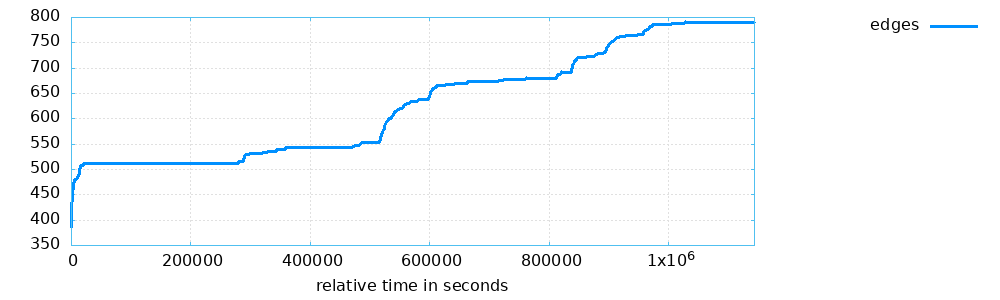
\includegraphics[width=1\textwidth]{cov-pgf}
    \caption{Edge Coverage over Time when fuzz testing the software on the
    emulator with the Protocol Grammar Filter}
    \label{fig:cov-pgf}
\end{figure}

\begin{figure}[H]
    \centering
    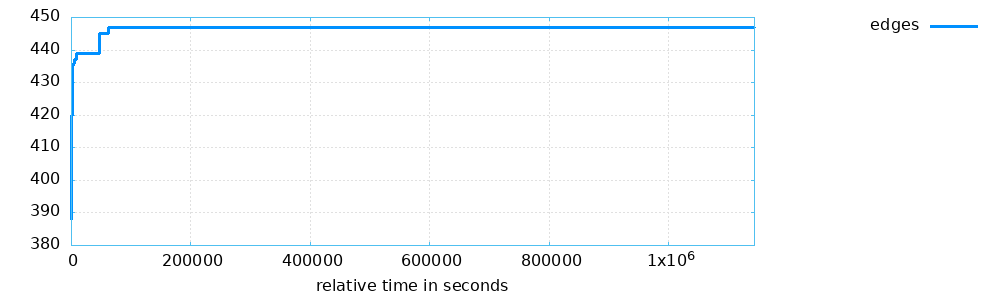
\includegraphics[width=1\textwidth]{cov-raw}
    \caption{Edge Coverage over Time when fuzz testing the software on the
    emulator with no input filtering}
    \label{fig:cov-raw}
\end{figure}

Initially, both \autoref{fig:cov-raw} and \autoref{fig:cov-pgf} show that the
initial edge coverage results are similar for both raw and PGF input. However,
\autoref{fig:cov-pgf} shows that the edge coverage continues to steadily
increase using the PGF, while without the PGF no more coverage is achieved. The
figures show that by the end of the run, fuzzing with the PGF has covered
nearly double the number of edges than fuzzing with raw input.

Additionally, the input files generated by AFL++ can be replayed through the
emulator to generate instruction coverage metrics. This coverage can be
presented as a percentage of the total number of instructions covered by the
generated input data. Using AFL++ without the protocol grammar filter achieved
70.4\% instruction coverage after the run was complete, while using the PGF
achieved 79.5\% instruction coverage.

The instruction coverage metrics for the PGF are not that much higher than
without. It is likely that the remaining 20\% of instructions not covered by
either method are not able to be covered by only fuzz testing the spacepacket
interface. This unreachable code might include guard conditions at start-up or
when initialising the RTOS. Additionally, this may include DBC asserts used
liberally throughout the FSW. For example, it may be impossible to fail a null
pointer check if all pointers are initialised and statically allocated, as they
should have been in the FSW. Furthermore, the similarity in instruction
coverage could be explained by the code size of all the application layer
implementation being relatively small compared to the HAL, start-up code and
RTOS, which would be covered regardless of any spacepacket input. This is
further demonstrated by the initial coverage achieved by the fuzzer being
relatively high. For both the raw and PGF results, the initial instruction
coverage percentage after running the first input is 65.23\%. Therefore, the
relative increase in coverage shown by with the PGF is two times greater than
the coverage achieved without using it, which should show its utility.

It also may be the case that the instructions covered using the PGF are not the
same as using raw input. The PGF greatly helps the fuzzer to create well formed
inputs that can be deframed correctly and have valid checksums, and is
therefore more able to test the application code. The raw fuzzer would struggle
to generate validly framed data with correct checksums. However, the PGF
currently does not allow the fuzzer to mutate data to cover different error
conditions in the deframing functions, while the raw fuzzer would be able to.
As the PGF can only introduce known errors into the protocol, the current
design of the PGF is a compromise between comprehensive fuzzing and specific
manually designed system testing. It is therefore likely that modifying the PGF
to allow more error conditions that can be controlled by the fuzzer would lead
to more effective fuzzing.

As UnicornAFL took a long time to run, it was left for long periods with bugs
only analysed after. This approach was less useful for testing during
development, as one logical error caused a large number of inputs to be
incorrectly executed in the fuzzer. Any other results beyond that bug had to be
discarded, and the process started again. It would seem using fuzzing tools
like AFL++ is more appropriate for software that has already been extensively
tested and completed its development. Then the fuzzer could be used to try and
catch any remaining errors that are hard to uncover with manual testing, rather
than as a tool during development for verifying new code.

% AFL had to set the timeout value higher as the emulator takes so long to run.
% FIXME

% coverage guided fuzzing implementation, explain AFL, show some screen shots.
% - difficulty with taking a long time to fuzz?
% - discuss potential improvements such as parallel builds
% - reducing fuzzing area (i.e target specific functions)
% - fuzzing potential more useful for analysis or verification of finished software, rather than software still in development.
% - fuzzing results somewhat invalidated after any changes, which is an issue when there is churn in implementation, and while fuzzing takes 6 days + to get meaningful coverage

% Present Fuzzing Results, show coverage graphs
% tradeoffs between grammar fuzzing and normal data
% - checksum and frameing means more data gets through to application
% - have to inject known errors to get coverage in protocol layer (e.g. invalid headers), reduces the effectiveness of fuzzing for finding bugs/vulnerabilities in this area.

\end{document}
